
%%% Local Variables: 
%%% mode: latex
%%% TeX-master: t
%%% End: 

\chapter{相关工作}
\label{chap:background}

随着互联网应用需求的不断增长,数据中心所需要的服务器数量也在飞速增长中。
受到电力供应、冷却系统以及占地面积等客观因素的影响,
服务器规模并不能够无限制的扩大,即将成为数据中心发展的瓶颈;
另一方面,当前的数据中心设计并不是最优的,
典型表现在于其资源利用率非常低,如前文所述只有6\%$\sim$12\%。
通过改进数据中心设计,提高服务器资源利用率,是解决数据中心扩展性问题的一个途径。
资源共享是提高资源利用率的主要手段,但它也会带来应用服务质量下降的问题,
现有大量研究尝试解决资源利用率与应用服务质量相冲突的问题,
本节对这些相关工作进行介绍。

\section{服务器资源共享}

通过服务器资源共享,将多个应用运行在同一服务器,是提高服务器资源利用率最为直接的方式。
但不同应用对操作系统、运行时环境等需求各不相同,无法直接实现应用混合部署;
即使是运行时环境兼容的两个应用,部署在同一台服务器后,
对某一应用配置的修改都可能会对另一个应用的运行造成影响;
同时,由于数据中心应用来自于不同的用户,混合部署还可能存在隐私与安全性问题,
造成应用数据信息的泄漏。
为解决以上问题,数据中心需要提供一种有效的资源隔离技术,
通过将应用运行在相互隔离的环境中,实现安全可靠的混合部署。
在服务器领域,当前流行的虚拟化与容器技术提供了这样的隔离环境。

% 虚拟化
虚拟化技术最初由IBM在20世纪60年代提出,
当时提出虚拟化的目的是为了提供系统的向后兼容性,以简化用户编程,
而后虚拟化一直是大型机基本的使用方式。
在此基础上IBM提出了逻辑分区(LPAR)\cite{IBM_LPAR:2007}技术,
该技术使得1台计算机能够像2台或更多台独立计算机一样运行,
提供了硬件层次的隔离,
其他一些厂商如Hitachi\cite{hitachi-lpar}和Sun(Oracle)\cite{LDom}也提供了类似的解决方案。

VMware最先将虚拟化技术引入到基于x86的PC服务器领域,
由于当时x86架构并没有提供任何虚拟化的支持,
VMware使用二进制翻译\cite{vmware-compare-hw-sw:2006}
的方式实现操作系统内核中不支持虚拟化的指令执行,
如图\ref{fig:compare-of-virt}(a)所示,实现对用户操作系统透明的虚拟化方案。
这种基于二进制翻译的全虚拟化方案性能存在问题,
因此Xen提出了半虚拟化(para-virtualization)\cite{barham_xen_2003}的概念,
通过修改客户机操作系统,直接使用Hypercall的方式调用hypervisor
(如图\ref{fig:compare-of-virt}(b)所示),提高系统性能。
在虚拟化产业发展起来后,各个硬件厂商分别推出新的硬件功能以更好的支持虚拟化,
如Intel的VT-x技术和AMD的AMD-V技术,如图\ref{fig:compare-of-virt}(c)所示,
硬件辅助虚拟化逐渐成为主流。
随着虚拟化技术性能的不断提高,当前在PC服务器领域,
虚拟化技术已经成为数据中心内被普遍使用的技术。

\begin{figure}[t]
  \centering
  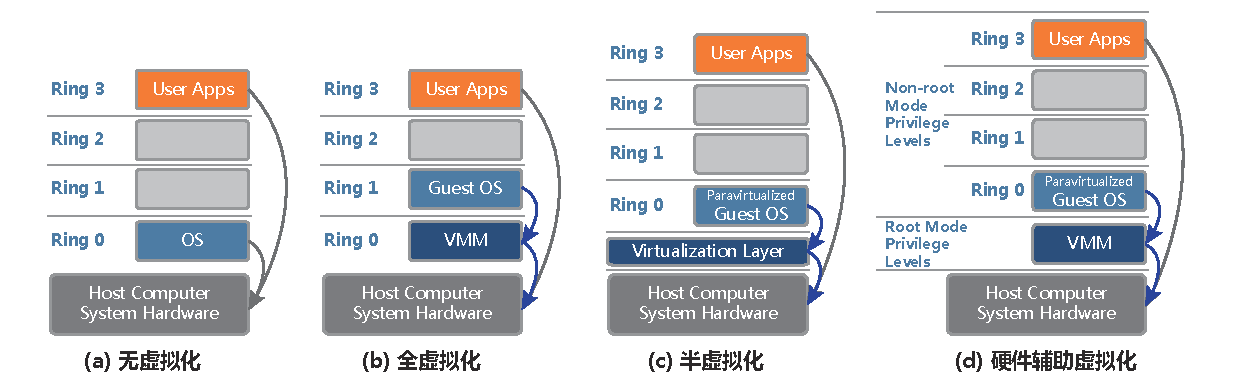
\includegraphics[width=\textwidth]{bg/compare-of-virtualization}
  \caption[3种不同类型虚拟化技术的对比]{3种不同类型虚拟化技术的对比:
    (a)无虚拟化,直接执行用户与OS请求;
    (b)全虚拟化,直接执行用户请求,二进制翻译执行OS请求;
    (c)半虚拟化,直接执行用户请求,修改GuestOS通过Hypercall实现特权指令;
    (d)硬件辅助虚拟化,直接执行用户请求,硬件支持OS特权指令直接陷入到VMM。}
  \label{fig:compare-of-virt}
\end{figure}

%容器轻量级虚拟化
基于容器的轻量级虚拟化是另一种流行的服务器融合技术,
与虚拟机抽象类似,不同容器之间以及容器与主机操作系统之间是相互隔离的,
但它们共享一份操作系统内核,可以有效的提高资源利用率。
以Docker为例(如图\ref{fig:docker-overview}),
用户的应用与依赖的运行时环境被打包为一个容器,
容器之间使用Linux内核的LXC\cite{lxc}机制实现名字空间隔离,
同时使用Control Group\cite{cgroup}实现资源控制。
与虚拟化技术相比,容器技术最大的优点是它具有更少的资源占用,以及更快的启动时间,
因此也被普遍运行在数据中心场景中。

\begin{figure}[htb]
  \centering
  \begin{minipage}{0.75\textwidth}
    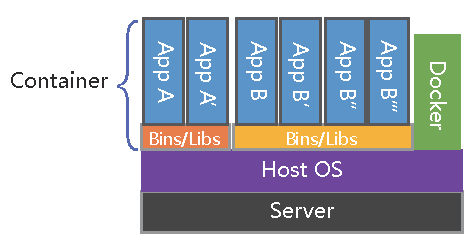
\includegraphics[width=0.75\textwidth]{bg/docker-overview}
    \caption[容器虚拟化结构示意(Docker)]{容器虚拟化结构示意(Docker):
      容器中包含应用及其依赖的运行时环境,容器之间相互隔离但它们共享同一份操作系统内核。}
    \label{fig:docker-overview}
  \end{minipage}
\end{figure}

% TODO:各种服务器融合技术对比

Google是最早在其数据中心实现多应用混合部署,他们的混合部署方案是基于cgroup的容器技术。
前文所提到的Google将离线数据中心资源利用率提高到75\%,
应用混合部署在其中起到了关键作用。
资源共享能够提高利用率,但它也带来了应用之间由于资源竞争产生的干扰。
研究\cite{}中发现虚拟化会带来严重的性能开销,\cite{}发现这些技术对干扰隔离不好,
会造成应用失去响应,IBM发现虚拟化虽然提高利用率降低硬件成本,
但性能下降所造成的收益下降,使得虚拟化成本要高于直接运行\cite{}。
这也是为什么Google并没有在其在线应用数据中心采取相同的资源共享的原因。


\section{服务质量评价指标}



\section{软件服务质量保障技术}


\subsection{任务调度}

调度的基础是对干扰进行评估。
对干扰进行评估是一个重要工作, measuring 2012做了这样的事情,评估了不同应用之间的干扰。

通过服务器共享,存在不同应用组合,由于干扰存在的可能,为保障关键应用QoS,通常会过量预留资源。
但有些时候这样过量预留是没有必要的,(Bubble-up里有说明),
在众多应用中寻找无干扰的任务组合是一个耗时工作,$O(N^2)$。
Bubble-UP提供了一种精确预测干扰的方法,为调度提供数据基础。


之前的工作都是针对长时运行的应用,通过对应用进行分析建模,得出其干扰特性,然后进行调度,
Paragon针对复杂变化应用,进行调度,其特殊是能够快速精确的识别出应用特征,使用离线建模在线预测的方式。

Quasar用户指定的资源不准确,造成资源浪费。通过用户指定需求,由系统自动分配资源,实现资源管理。以性能为中心的资源调度(非任务调度,放到后面会更好)。


虽然存在潜在的竞争,但资源需求不同的应用在混合运行时,却不一定会带来干扰。如图\ref{}所示,研究\cite{}表明,一些应用在混合运行时并没有产生严重的干扰。基于该观察,一些研究\cite{}尝试从作业调度的角度来解决共享与干扰的问题。如Bubble-Up\cite{}工作,使用模拟的bubble性能,来带来应用对其它应用干扰程度,通过profiling的方式,确定不同应用的行为,选择相同干扰较小的应用进行混合,解决干扰问题。Paragon\cite{}也是一样,使用XXX的方式,实现作业调度。Quasar\cite{}也是一个作业调度的工作,通过XXX,解决XXX。这类解决方案的核心是数据中心存在大量可供调度的应用,通过恰当的作业调度与放置,能够实现干扰最小化。该方案的问题在于,需要对应用行为特征进行分析,才能做出正确的调度决策,但数据中心应用众多,不断变化,没有稳定的运行集合,对这些应用进行分析耗时,且不现实;大部分应用短时运行,分析所花费的时间要大于运行时间。因此,此类方案只能适用于作业相对稳定、且长时运行的场景。

收益成本低过低, 当前数据中心\cite{mesos,openstack}并没有采用这种基于QoS的调度,而是使用简单的基于资源的调度。更多需要考虑在这样的场景下如何保障应用服务质量。

\subsection{执行控制}
ReQoS, DVFS, Bubble-Flux


\subsection{资源隔离}
cgroup, page-coloring, CAT



\subsubsection{资源管理与服务质量保障}

软硬件资源的竞争在整个系统栈中存在,
表\ref{tab:contention}列出了不同层次上可能存在的竞争点,
以及在不同层次上消除竞争点的相关工作。
Google和Twitter等互联网公司也尝试改进数据中心管理系统架构,
实现服务器资源利用率与应用服务质量之间的平衡,
一些典型系统包括:Borg\cite{borg:2015}、Omega\cite{Schwarzkopf_omega_2013}和
Mesos\cite{Hindman:2011:Mesos}。
另外一些研究工作尝试使用分布式技术或操作系统内核优化技术实现应用服务质量保障,
如多级优先级策略\cite{Reiss_googletrace_2012}、
调度方法\cite{delimitrou_paragon:_2013, delimitrou_quasar:_2014, mars_heterogeneity_2011,
kozyrakis_reconciling_2014, Novakovi:ATC2013}、
backup-request\cite{dean_tail_2013},cgroup\cite{cgroup}和容器技术\cite{lxc}。 
本节主要关注节点内资源管理与服务质量保障的相关研究,包括软件和硬件两个方面。

\begin{table}[hb]
  \centering
  \caption{资源管理与服务质量保障相关工作中识别出的竞争点}
  \label{tab:contention}
  \begin{tabular}{p{0.15\textwidth}p{0.75\textwidth}}
    \toprule[1.5pt]
      {\heiti 层次}     & {\heiti 竞争点}                                                                                      \\
    \midrule[1pt]
      数据中心          & Global file system \cite{dean_tail_2013}                                                                        \\
      应用层            & Background daemon \cite{dean_tail_2013}, backup job \cite{yu_profiling_2011,dean_tail_2013}                     \\
      网络协议栈        & Nagle's algorithm, limited buffers, delayed ACK caused RTO \cite{yu_profiling_2011},
                          TCP congestion control \cite{alizadeh_data_2010,dong_less_2013},
                          packet scheduling \cite{vamanan_deadline-aware_2012,wilson_better_2011,zats_detail:_2012,hong_finishing_2012},
                          kernel sockets \cite{kozyrakis_reconciling_2014}                                                                \\
      操作系统内核      & Lock contention \cite{Kapoor:2012:Chronos}, context switch, kernel scheduling,
                          SMT load imbalance and IRQ imbalance \cite{kozyrakis_reconciling_2014}                                          \\
      虚拟化层          & Virtual machine scheduling \cite{Xu:2013:Bobtail:,wang_impact_2010, Xu:2013:SMALL},
                          network bandwidth \cite{wang_impact_2010,shieh_sharing_2011,Xu:2013:SMALL,jeyakumar_eyeq:_2013}                 \\
      硬件              & Shared caches \cite{kozyrakis_reconciling_2014,Tang:2011:ISCA,kasture_ubik:_2014,sanchez_vantage:_2011,sanchez_zcache:_2010,qureshi_utility-based_2006,DelimitrouK13:ibench},
                          memory \cite{Tang:2011:ISCA,yang_bubble-flux:_2013,muralidhara_reducing_2011,DelimitrouK13:ibench},
                          NIC \cite{Radhakrishnan:2014:SENIC},
                          I/O \cite{mesnier_differentiated_2011,DelimitrouK13:ibench}                                                     \\
    \bottomrule[1.5pt]
  \end{tabular}
\end{table}


\subsubsection{软件服务质量保障技术}


针对该问题,Bubble-Up的后续工作Bubble-Flux提出在线冲突检测与隔离机制,通过周期运行资源检测的方式,发现冲突,在发生干扰时使用名为PiPo的方式对低优先级应用的执行进行控制,具体是采用linux的信号机制暂时低优级应用的执行。ReQoS\cite{}也采取控制低优先级应用执行的方式,实现干扰控制,它通过编译的方式识别出低优级应用中可能会对内存子系统产生干扰的代码段,并在其中插入hook;在运行时环境中对干扰进行检测,发现干扰时,通过之间插入的hook,对低优先级应用的执行进行控制,降低干扰的影响。

以上两个方案的核心思路是“源抑制(source throttling)”,在检测到干扰发生时,对低优级应用的执行进行控制,降低其对资源的使用(主要是Cache/memory内存子系统)。其他一些工作使用硬件支持也实现了源抑制的功能,如研究\cite{}使用clock modular的技术,降低低优先级应用所在核的频率,工作\cite{}使用DVFS也可以用作相同的目的。

内存子系统对应用性能影响最大,包括Cache和Memory。对于Cache资源的竞争,主要体现在对基容量竞争上,基于该观察,工作\cite{}提出需要对缓存容量进行划分,比混着用要好。工作\cite{}利用Page coloring的方式,对XXX,通过XXX,在软件层次实现容量划分,不过该工作对于最新的处理器无效,因为使用了复杂的hash,且不公开,无法得知具体的映射信息。处理器厂商也意识到多应用cache竞争问题的重要性,intel在其处理器中增加了缓存容量划分的功能,Berkely团队对该功能进行的评估\cite{},发现通过划分的方式,能够有效的隔离cache层次上的干扰。

总结软件层次的工作,其核心控制应用执行及其所占用的资源,控制粒度很粗,一但发生干扰,完全没有办法。CAT是一种新的思路,在硬件上支持资源管理,并将接口暴露给软件控制,后文讨论在硬件上解决干扰问题。同时软硬件协同的相关工作将在下一节中介绍。


\section{硬件服务质量保障技术}

如前文,Cache和Memory是两上影响应用性能最重要的资源,本部分讨论在这两类资源上实现服务质量保障的技术。


\subsection{Cache上的服务质量保障技术}

容量是Cache性能的主要因此,CAT是Intel处理器上第一个对cache容量进行划分的技术,实现了按way划分的功能,同时其CMT技术,实现按应用区分的cache性能监控,基于这两个工作,可以实现cache层次上资源管理。Cache路划分最早由\cite{}提出,但这种划分方式只能以路为粒度进行划分,而一般处理器路数不多(目前intel处理器普遍只有24路),划分的粒度与支持的应用数会受到限制;划分后关联度下降也会造成cache性能下降。

对于划分粒度问题,后续一些研究提出更为细粒度的划分机制,如\cite{}提出按set划分的方式,\cite{}按block为粒度的划分;对于关联度下降的问题,ZCache\cite{}提出一种新的cache设计,将缓存路与关联度解耦,提高关联度为缓存容量划分提供更大的空间,Vantage\cite{}基于该缓存实现了一种细粒度的缓存容量划分方案。

Cache划分的另一个问题是容量分配问题,UCP提出一种基于使用的容量划分策略,通过UMON实现监控,获取不同路的性能,选择最优的方案;Ubik和Jigsaw基于该策略实现了不同的cache资源管理方案。

\subsection{内存上的服务质量保障技术}

针对内存控制器上的竞争,Muralidhara 等人提出了一种应用感知的内存通道划分技术 MCP[21],用于降低应用在内存子系统的干扰。以 CMU 的 Onur Mutlu 为代表的一些研究提出一系列调度算法 [67–70] 以缓解内存控制器的不公平问题,从而提高系统吞吐量以及服务质量。


这件事情,硬件不能独立完成,因为它没有应用的信息,需要软硬件协同,在下节介绍。

但这些算法是固化的,并不能针对某个应用进行调节,灵活性较差。

硬件区分,PARD提出标签化地址空间

硬件资源统一管理,控制平面


\section{服务质量保障框架}

因为软件知道应用需求,硬件能够对资源进行细粒度控制,QoS保障需要软硬件协同。在实现QoS策略与机制前,需要首先定义QoS指标。Iyer等人cite{}提出了3种QoS目标,分别是: 资源用量指标(Resource Usage Metrics,RUM),定义应用的资源使用,如Cache容量即为RUM指标;资源性能指标(Resource Performance  Metrics,RPM),定义资源性能,如Cache缺失率;整体性能指标(Overall Performance Metrics,OPM),指示程序的整体性能,如IPC。大多数早期QoS工作\cite{}都使用以IPC为代表的OPM作为QoS指标。针对数据中心场景,OPM中需要额外增加Tail-Latency指标,它是反映延迟敏感型在线应用性能的主要指标,工作如\cite{}都使用它作为QoS指标。资源利用率实际对应的是RUM指标,因此本文所要解决的问题就是实现RUM与OPM的平衡。

CoQoS是目前对QoS保障框架描述最为完整的工作,其提出QoS保障要分为三个部分,分别是CoS Assignment、CoS Mapping、和CoS-Based Resource Mgmt。其中第一阶段用于,XXX;第二阶段用于XXX;第三阶段用于XXX。对比本文工作,本文所提出的PARD体系结构以逻辑域为粒度保障QoS,通过标签寄存器标记硬件请求,使用控制平面进行标签与资源分配映射,使用PRM集中式管理所有资源。

Heracles是最相似的,

Rafique提出一种OS/Cache协同的方案。


%% Comment for remove
\iffalse

\textbf{软件服务质量保障技术}\quad

在软件层次上主要采用隔离与调度2个方法实现服务质量保障。

%% 虚拟化可以提供隔离,但性能上很差,主要是硬件层次会有干扰,无法实现隔离
%虚拟化技术能够提供一定程度的
%
%

% 页着色可以通过软件实现cache和dram的划分,但不太灵活
页着色技术(page coloring)是一种以软件方式控制内存物理页映射的方法,
通常被用作共享末级缓存与DRAM的划分,其核心思路是通过控制地址映射信息实现硬件资源的管理。
一些研究利用该技术实现共享末级缓存划分\cite{lin_gaining_2008, tam_managing_2007}
来解决应用之间缓存竞争问题,
或在虚拟化场景下实现缓存划分\cite{Jin2009, Chen2010, Wang2012};
还有一些研究\cite{liu_software_2012}使用该技术实现DRAM的bank划分,
来消除bank级的干扰与竞争,或实现DRAM与末级缓存的协作式划分\cite{Liu:2014:ISCA}。
但该技术存在2个方面的问题:
首先,当应用负载发生变化时,需要在内核中重新组织空闲页链表并进行必要的页面迁移,
这需要非常大的软件开销;
更为严重的是,目前的处理器通常使用复杂的哈希算法实现从物理地址到cache index的映射
(如Intel的SandyBridge架构),
而这些哈希算法通常并不会公开,因此在这样的系统上实现页着色是不现实的。

%从调度的角度也有一些研究,但都是ad-hoc的工作,无法普及
在软件调度方面也存在大量研究,
例如,CAER框架\cite{mars_contention_2010}是一种竞争感知的轻量级运行时环境,
能在提高利用率的同时减少由于片上或片外资源的竞争所引起跨核应用之间的干扰;
CiPE框架\cite{mars_directly_2011}可以直接测量和量化多核结构下应用的跨核干扰敏感度,
并以此为依据进行作业调度。
Jason Mars等人设计的Bubble-Up\cite{mars_bubble-up:_2011}机制,
通过使用气泡(Bubble)来代表内存子系统的可变压力情况,
能准确预测在内存子系统中竞争共享资源而导致的性能下降,通过离线分析来决定最优的应用混合,
Bubble-Flex\cite{yang_bubble-flux:_2013}工作在Bubble-Up离线的基础上,实现了在线的QoS管理。
ReQoS\cite{tang_reqos:_2013}提供了一种编译技术与运行时环境相结合的方法,
通过编译的方法标识出低优先级应用中可能引起竞争的代码段,
通过运行时环境调节低应用级应用的执行来确保这些代码段不会对高优先级应用的服务质量造成影响。
以上这些工作虽然能够缓解服务质量与资源利用率的冲突,
但它们的解决方案都只能针对特定的场景,不具有通用性。


\textbf{硬件服务质量保障技术}\quad

由于单纯使用软件技术无法解决应用在硬件层次的干扰,
目前学术界和工业界在硬件层次上提出一系列方案,解决干扰问题。
其中以处理器末级缓存与内存控制器上的硬件方案居多。

针对处理器末级缓存容量的竞争,Kasture和Sanchez提出的Ubik\cite{kasture_ubik:_2014},
通过识别和利用延迟敏感型应用瞬时性的特点,调整缓存容量划分策略,来保证目标长尾延迟。
UCP\cite{qureshi_utility-based_2006}提出了一种应用缓存容量需求的探测方法,
为应用分配收益最大的缓存划分方案。
由于受到工艺、面积以及能耗的限制,目前的常见处理器末级缓存关联度最大只有24,
不足以分配给其上运行的应用,
针对该问题ZCache\cite{sanchez_zcache:_2010}提出了一种新的缓存方法,将缓存路与关联度解耦,
提高关联度为缓存容量划分提供更大的空间,
Vantage\cite{sanchez_vantage:_2011}基于该缓存设计实现了一种细粒度的缓存容量划分方案。

%Kasture and Sanchez propose Ubik \cite{kasture_ubik:_2014},
%a cache partitioning policy that characterizes and leverages the transient
%behavior of latency-critical applications to maintain their target tail latency.
%Vantage \cite{sanchez_vantage:_2011} implements fine-grained cache partitioning
%using the statistical properties of Zcaches \cite{sanchez_zcache:_2010}.
%Utility-based cache partitioning (UCP) \cite{qureshi_utility-based_2006}
%strictly partitions the shared cache depending on the benefit of allocating
%different number of ways to each application.

针对内存控制器上的竞争,
Muralidhara等人提出了一种应用感知的内存通道划分技术MCP\cite{muralidhara_reducing_2011},
用于降低应用在内存子系统的干扰。
以CMU的Onur Mutlu为代表的一些研究提出一系列调度算法\cite{mutlu_stall-time_2007,
mutlu_parallelism-aware_2008, kim_atlas:_2010, kim_thread_2010}
以缓解内存控制器的不公平问题,从而提高系统吞吐量以及服务质量。
但这些算法是固化的,并不能针对某个应用进行调节,灵活性较差。

除硬件层次的划分与调度外,Andrew Herdrich等人\cite{herdrich_rate-based_2009}
发现了用于功耗管理的处理器限速技术(如DVFS),
能够应用到QoS领域用于实现处理器末级缓存与内存控制器上的竞争管理。
其基本方法是当正在运行的低优先级任务由于资源竞争争而干扰了高优先级任务的性能时,
就减缓核心的处理速率,通过请求抑制的方法缓解低优先级任务对共享资源的竞争。

在QoS保障框架方面,
Rafique等人提出了一种操作系统驱动的缓存容量划分机制\cite{Rafique:2006:ASO},
通过标记Cache访问请求来允许操作系统根据标记对Cache容量划分进行管理。
Sharifi等人进一步提出了一种基于反馈的控制架构\cite{sharifi_mete:_2011},
以实现端到端的片上资源管理。
Ravi Iyer提出了一种保障CMP体系结构上缓存Qos的管理框架CQoS\cite{iyer_cqos:_2004},
将QoS工作分为3个阶段,即优先级分类(Priority Classification)、
优先级分配(Priority Assignment)和优先级实现(Priority Enforcement)。
然而,该工作只设计了QoS保障的框架,而并没有详细描述具体策略和软硬件支持。
后续的工作\cite{iyer_qos_2007, li_coqos:_2011, li_dynamic_2012}实现了
基于class-of-service的QoS架构(CoQoS),通过为片上请求标记优先级的方式,
实现基于优先级的Cache/DRAM/NoC请求调度。

\fi

\section{计算机网络与服务质量}
\label{sec:background:sdn}

服务质量问题在计算网络领域存在大量研究,从原型上来说主要分为3类。
第1类是资源过量分配,根据峰值需要分配网络资源,实现服务质量保障;
第2类是以集成服务(integrated services,IntServ)\cite{IntServ}和
区分化服务(differentiated services,DiffServ)\cite{DiffServ}
为代表的共享网络环境下的服务质量保障方法,
该方法的核心思路是在网络包中增加应用区分的标签,
可以是基于单个应用(IntServ)或基于服务类型(DiffServ),
以标签为粒度在网络链路上预留资源,实现服务质量保障。
第3类是以软件定义网络SDN\cite{SDN}为代表的可编程网络架构,
能够根据应用需求的变化,通过可编程的方式实现网络拓扑的调整,
同样能够实现服务质量保障。

当前数据中心区分在线应用与离线应用的方法,
映射到网络领域可以被看做是第1类和第2类方案的结合:
使用较粗的粒度对应用进行区分(在线、离线),
并为在线作业过量分配资源,以保障其服务质量。
从网络领域的经验来看,该方案会造成严重的资源浪费,
事实也是正是如此,数据中心只有6\%$\sim$12\%的资源利用率。
要解决数据中心资源利用率与服务质量冲突,可以从网络领域中借鉴更多的思路,
包括细粒度的应用区分、以及可编程的网络管理,
本文所提出的资源管理可编程体系结构正是基于以上思路。
通过在计算机体系结构内实现应用区分与可编程的资源管理,
来解决数据中心资源利用率与服务质量的冲突。

%\begin{figure}[tbh]
%  \centering
%  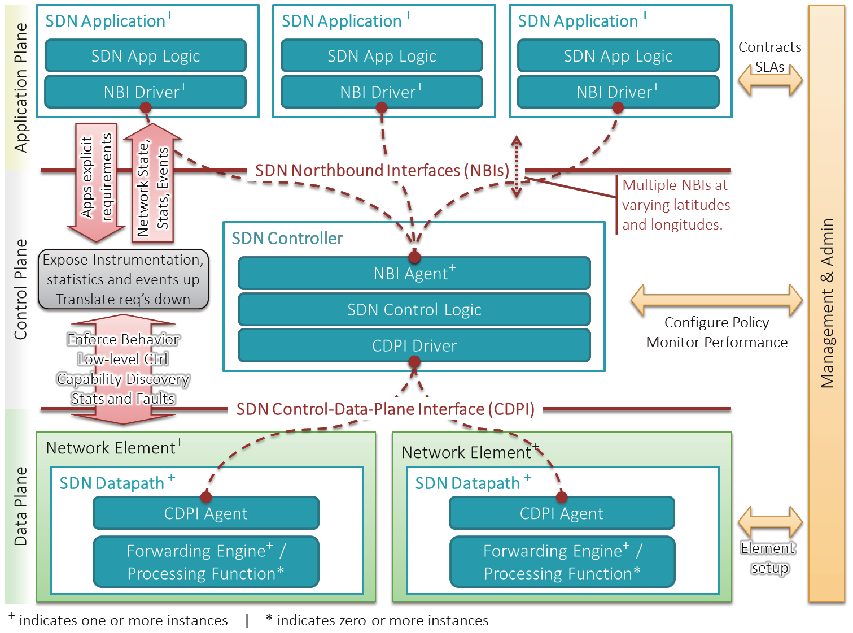
\includegraphics{arch/sdn-arch.pdf}
%  \caption{软件定义网络SDN架构}
%  \label{fig:pard-arch-outline}
%\end{figure}


\section{本章小结}

本章首先介绍了本文的研究背景与问题,
即新计算模式下数据中心面临应用服务质量与资源利用率相冲突的问题,
并从软件和硬件两个角度总结针对该问题的相关研究。
从现有技术来看,单节点内服务质量保障技术的不足,导致节点内应用相互干扰严重,
已经成为目前数据中心整体服务质量保障的短板,是成为长尾延迟现象的主要因素之一。
单纯从软件或硬件层次无法根本解决该问题,而是需要跨层次协同设计。
而软硬件协同设计的关键在于``应用如何表达服务质量(QoS)目标并且让底层的硬件、操作
系统以及虚拟层共同工作来保障它们''\cite{21st_architecture}。
本文后续章节将围绕该问题讨论如何设计一种新型的体系结构,
通过软硬件协同的方式解决数据中心当前面临的这一难题。

